%!TEX root = ../main.tex



\newcommand{\Titel}{Projektplan}
%!TEX root = ../main.tex

\begin{titlepage}
	\begin{center}
		\vspace*{-2.5cm}
		\hfill	
\includegraphics[width=5cm]{images/dhbw.png}\\[5cm]
		
		{\Huge \scshape \Titel}\\[1cm]
		{\large für die Erstellung der Studienarbeit}\\[0.5cm]
		\vspace{1cm}
		
		%{\large von}\\[0.5cm]
		%{\large \Autor \ \& \AutorZwei}\\[1cm]
		
		\vfill
	\end{center}
	\begin{tabular}{l@{\hspace{2cm}}l}
		\bfseries Teilnehmer & \Teilnehmer      \\
		\bfseries Datum      & \DatumUndZeit      \\
		\bfseries Ort        & \Ort             \\
		\bfseries Thema      & \Thema           \\
		\bfseries Betreuer   & \Betreuer        \\
		\bfseries Kurs       & \Kursbezeichnung
	\end{tabular}
	
\end{titlepage}



\definecolor{literaturrecherche}{RGB}{97,136,88}
\definecolor{entwicklung}{RGB}{72,141,215}
\definecolor{dokumentation}{RGB}{212,103,57}
\definecolor{QS}{RGB}{216,172,71}


\section{Terminplan und Meilensteine}
Das Projekt wird nach der agilen Projektmanagement Methode SCRUM erarbeitet.
Deswegen werden die einzelnen Arbeitsschritte in Sprints unterteilt, die jeweils eine Woche dauern.
Die einzelnen Aufgaben in jedem Sprint sind in der nachfolgenden Tabelle zu sehen.

In der Tabelle sind die einzelnen Schritte mit Farbcode hinterlegt, die die Aufteilung in die folgenden Themenbereiche hervorheben: \textcolor{literaturrecherche}{\textbf{Literaturrecherche}}, \textcolor{entwicklung}{\textbf{Entwicklung}}, \textcolor{dokumentation}{\textbf{Dokumentation}} (beinhaltet die schriftliche Ausarbeitung der Studienarbeit), \textcolor{QS}{\textbf{Qualitätssichernde Maßnahmen}}.

Am Ende existiert ein zusätzlicher Puffer, um Verzögerungen abzufangen.


\begin{center}
	\makebox[\textwidth]{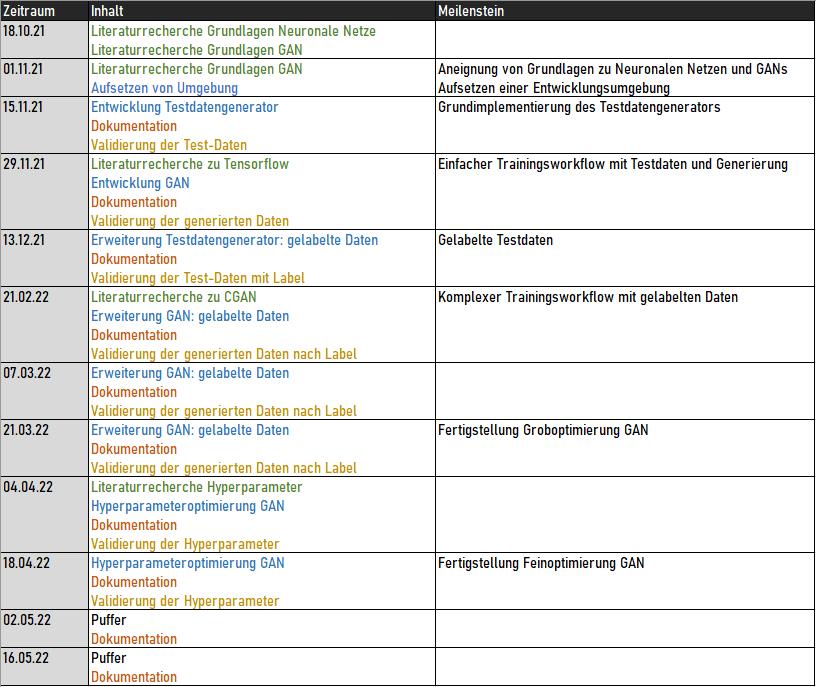
\includegraphics[width=1.0\textwidth]{allgemein/projektplan/Projektplan.png}}
\end{center}
